\documentclass[../main.tex]{subfiles}
\begin{document}

\section{Results}

\subsection {Genome organization and nucleotide composition}

\begin{figure}[htp]
    \centering
    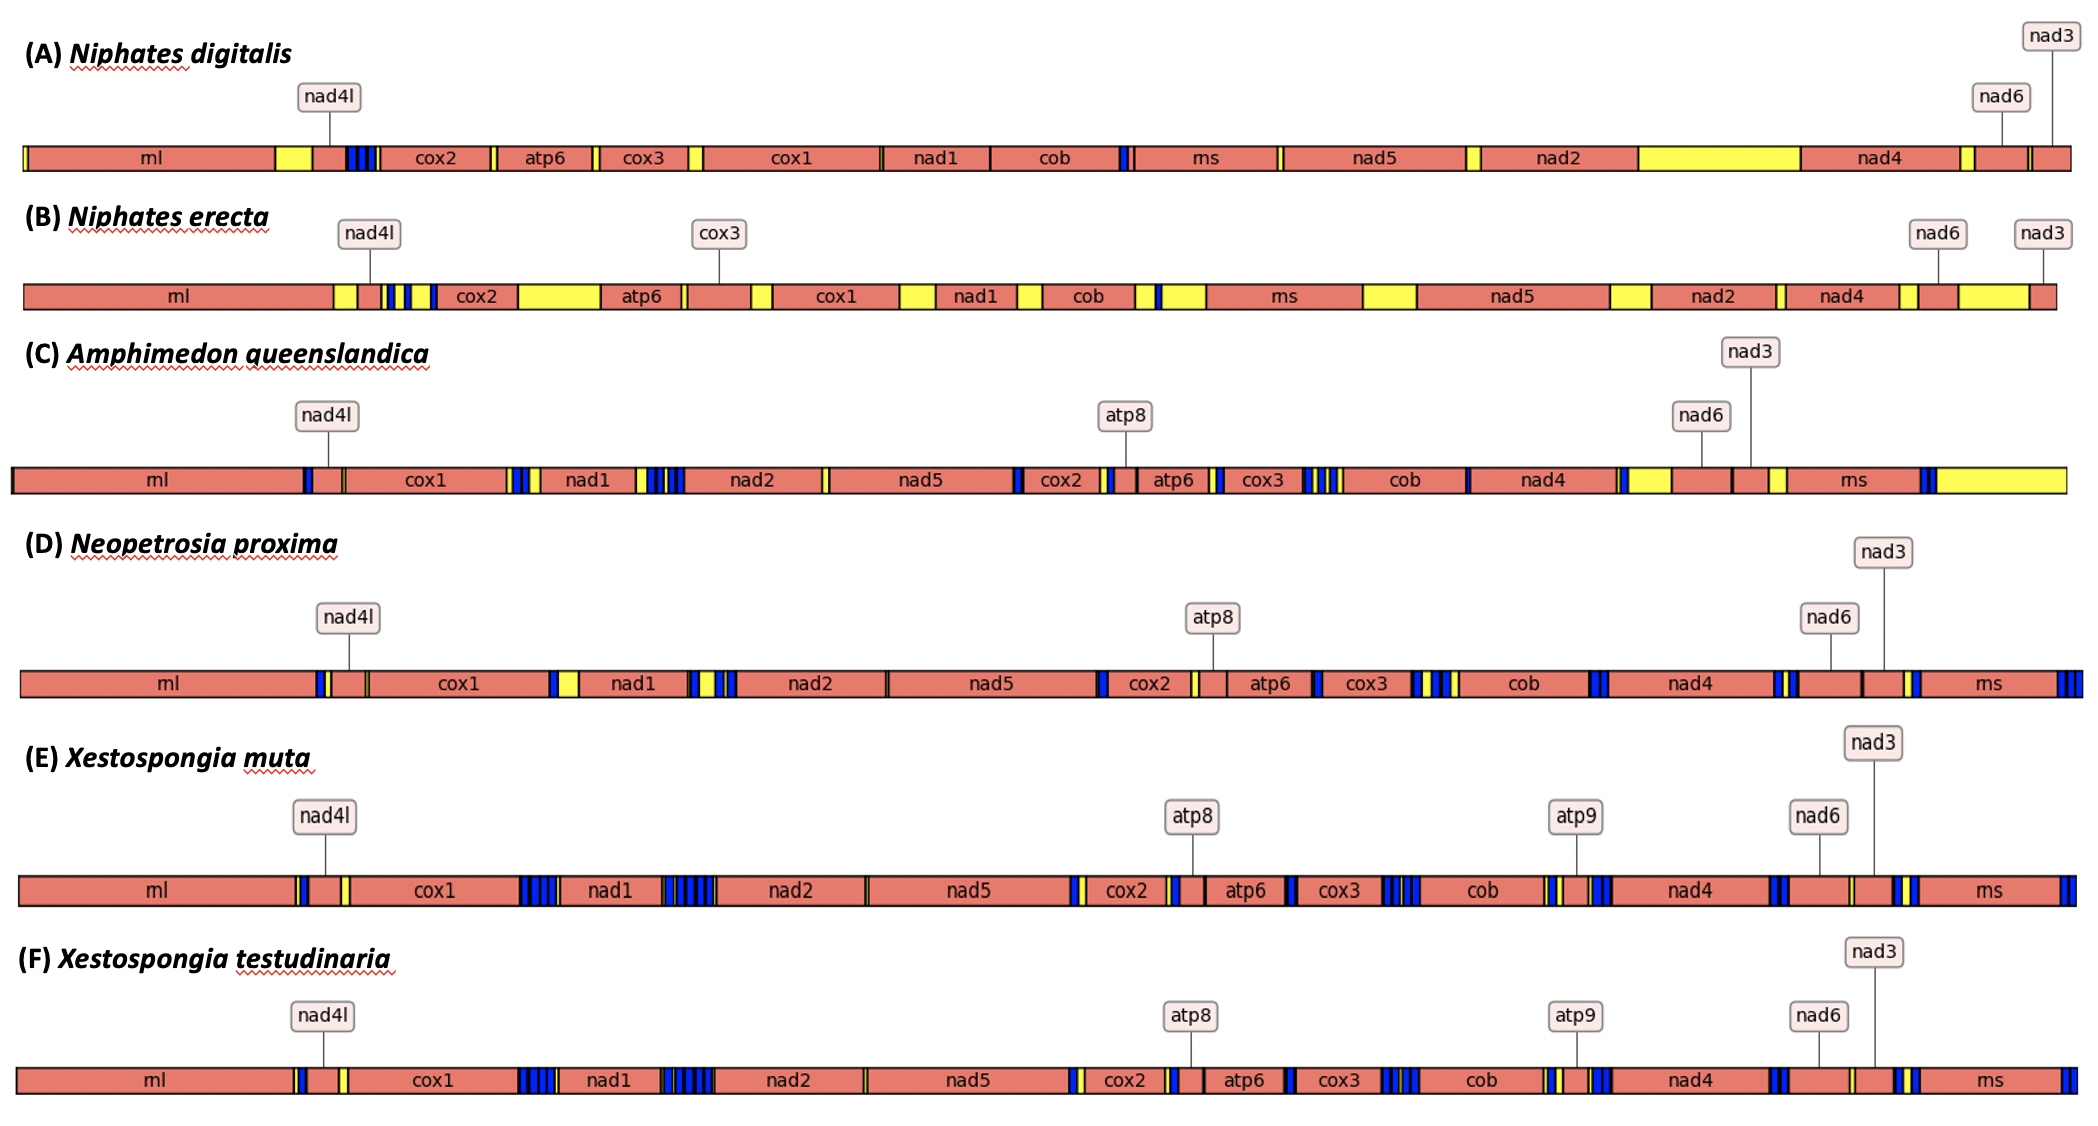
\includegraphics[width=1.0\textwidth]{Figures/figure 1 replace.png}
    \caption{Red are coding genes, blue is tRNA genes, and yellow are intergenic regions.}
\end{figure}

The mt-genomes of \emph{Niphates digitalis} and \emph{Niphates erecta} are reported here for the first time. They show a high degree of similarity after alignment and in further analysis are used interchangeably when data from the other species isn't available. This interchangeable use is also supported by their close phylogenetic relationship. These two genomes assemble into circular-mapping molecules, containing 12 protein-coding genes, two rRNA genes, and the same four tRNA genes (Figure 1a and Figure 1b) - tRNA(W), tRNA(Y), tRNA(M), and tRNA(I). The two mt-genomes show higher levels of intergenic regions compared to other Clade B sponges examined in this study, and have other subtle differences discussed below.

In addition to the mt-genomes of both \emph{Niphates} species, the mitochondrial genome of \emph{Neopetrosia proxima} is also reported here for the first time. Much the same as \emph{N. digitalis} and \emph{N. erecta}, this mt-genome assembles into a circular-mapping molecule, with 13 protein-coding genes, two rRNA genes, but retains 18 mt-tRNA genes, as opposed to the four retained in \emph{N. digitalis} and \emph{N. erecta}. It is missing tRNA(D), tRNA(L2), tRNA(Y), and tRNA(K). The differences in protein-coding gene content will be discussed below.

The mt-genomes of the other three species were previous published, and were curated from the literature. All three other species display variable protein-coding genes, variable tRNA genes, and intergenic genomes. Despite any differences, all six genomes displayed similar nucleotide composition (A+T content between 56\%-66\% and G+C content between 33\%-44\%, with the coding strand displaying AT nucleotide skew (Table 1). \emph{Amphimedon queenslandica} displayed the highest level of GC skew on the coding strand, with a GC percentage of 44\%; this also corresponds with a lower AT percentage (56\%) in this species. The five other species maintained a GC percentage of 33\%-36\%, and AT percentage of 63\%-66\%.

All genomes displayed a moderate degree of size variation (18-25.5kb, mean = 19.9kb). Five of the six genomes fell between 18kb and 20kb, with the outlier being \emph{Niphates erecta}, whose mt-genome totaled approximately 25.5kb. The increase in genome size for this species can be attributed to increase in the non-coding regions and stem-loop elements discussed later.

\begin{center}
\begin{tabular}{ |c|c|c|c| } 
 \hline
 \textbf{mt-Genome}& \textbf{AT Skew \%} & \textbf{GC Skew \%} & \textbf{mt-Genome Size (kb)}\\
 \hline

\emph{Niphates digitalis}  & 63.36 & 36.58 & 18,285\\
\hline
\emph{Niphates erecta} & 63.64 & 36.33 & 25,525\\
\hline
\emph{  Amphimedon queenslandica  } & 56.02 & 43.96 & 20,330\\
\hline
\emph{Neopetrosia proxima} & 66.00 & 33.78 & 17,967\\
\hline
\emph{Xestospongia muta} & 65.92 & 33.75 & 18,990\\
\hline
\emph{Xestospongia testudinaria} & 65.90 & 33.82 & 18,996\\
\hline
\end{tabular}
\end{center}

\subsection{Genome Content}
\subsubsection{Movement of \emph{atp9} from the mitochondria to the nucleus}
While the majority of protein-coding genes are well conserved in this clade, two genes seem to have been lost or moved to the nuclear genome. First, the gene \emph{atp9} was found to be missing in four of the six species - \emph{Amphimedon queenslandica}, \emph{Neopetrosia proxima}, \emph{Niphates digitalis}, and \emph{Niphates erecta}. However, \emph{atp9} is present in \emph{Xestospongia muta} and \emph{Xestospongia testudinaria}. It is well-known that \emph{atp9} has not been permanently lost in \emph{Amphimedon queenslandica}, but has instead moved to the nuclear genome. Considering the phylogenetic relationship of the four species with missing \emph{atp9}, the possibility of an ancestral move of \emph{atp9} was investigated. 

The potential movement of \emph{atp9} was not investigated in \emph{N. proxima} due to a lack of genomic and transcriptomic data; however, it was possible to examine this in \emph{N. digitalis} and \emph{N. erecta}. Using the nuclear \emph{atp9} sequence from \emph{A. queenslandica} as a query, several BLAST searches of an unpublished \emph{N. digitalis} nuclear genome revealed the presence of a corresponding \emph{atp9} sequence on two \emph{N. digitalis} nuclear contigs, with no other distinct matches. Much like the sequence seen in \emph{A. queenslandica}, the \emph{N. digitalis atp9} appeared to have gained at one intron, as the BLAST results return two segments on each \emph{N. digitalis} contig matching \emph{atp9}, with the two segments separated by 340 basepairs. 
Following this discovery, it was important to determine if the location where \emph{atp9} appears in the \emph{N. digitalis} nuclear genome is the same location \emph{atp9} appears in the \emph{A. queenlandica} nuclear genome. Both \emph{N. digitalis} contigs contain the \emph{atp9} sequences were aligned against the contig containing \emph{atp9} from the \emph{A. queenslandica} assembly and visualized on a dotplot (Figure 2). Large sections of each \emph{N. digitalis} contig were found to be be similar to parts of the \emph{A. queenslandica atp9} contig. The largest section, over 70,000 base pairs long, contained the alignment of \emph{atp9} between both species.

\begin{figure}[htp]
    \centering
    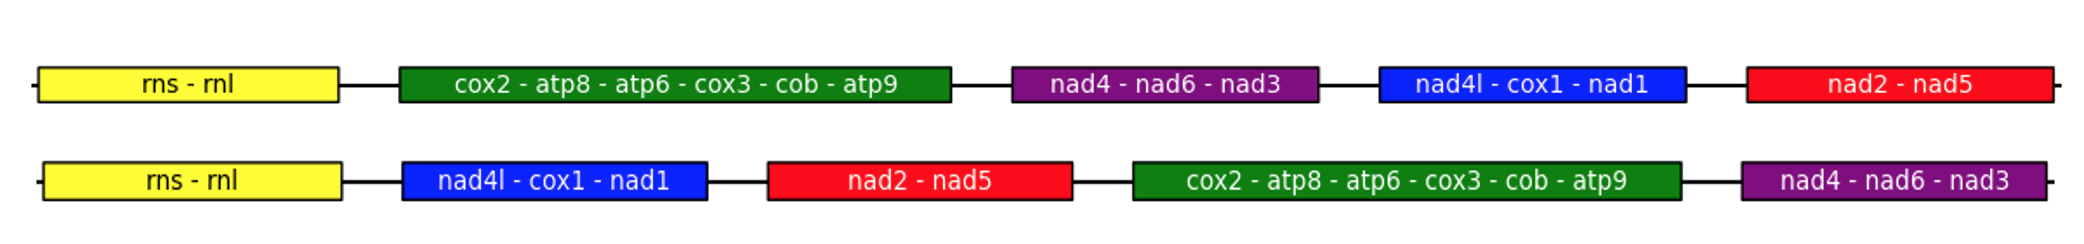
\includegraphics[width=1.0\textwidth]{Figures/figure 3.png}
    \caption{Dot plot showing sequence comparison between contigs containing \emph{atp9} in both \emph{Amphimedon queenslandica} (bottom axis) and \emph{Niphates digitalis} (left axis). Yellow dot represents match between both \emph{atp9} sequences.}
\end{figure}

While there is no nuclear genome for \emph{Niphates erecta}, it was possible to determine the presence of \emph{atp9} in the nuclear genome of this species as well. Using an unpublished transcriptome created in our lab, we were able to BLAST the transcripts for the \emph{atp9} sequence. As expected, transcripts of \emph{atp9} were recovered, and were identical in sequence to the nuclear copy found in \emph{Niphates digitalis}. Alignments of the nuclear copies from \emph{Amphimedon queenslandica}, \emph{Niphates digitalis}, the transcriptome copy from \emph{Niphates erecta}, and the mitochondrial sequence from \emph{Xestospongia muta} show that \emph{atp9} has acquired an upstream sequence in the three nuclear copies and is transcribed, as well as a downstream sequence seen in the genomic copies of \emph{Amphimedon queenslandica} and \emph{Niphates digitalis}, but is not seen in the transcribed copy found in \emph{Niphates erecta}. By comparing against the mitochondrial \emph{atp9} sequence seen in \emph{Xestospongia muta}, these additional appear to have been gained most movement to the nucleus.

\subsubsection{Movement of \emph{atp8} from the mitochondria to the nucleus}

In addition to the proposed movement of \emph{atp9} to the nuclear genome, \emph{Niphates digitalis} and \emph{Niphates erecta} have another lost mitochondrial gene, \emph{atp8}. This gene is found in the other four species of Clade B, including \emph{Amphimedon queenslandica} and \emph{Neopetrosia proxima}, which already show the loss of \emph{atp9}. It was once again proposed that \emph{atp8} underwent a similar fate to \emph{atp9} and moved to the nuclear genome. 

To investigate this hypothesis, the nuclear genome of \emph{Niphates digitalis} and the transcriptome of \emph{Niphates erecta} were searched for evidence of \emph{atp8}. BLAST searches of \emph{N. digitalis}'s nuclear genome returned no results under any parameters. In addition, BLAST searches of \emph{N. erecta}'s transcriptome also returned no results under any parameters. Thus, it does not appear that \emph{atp8} has been moved to the nuclear genome, and has been lost completely.

\subsection{Gene Order}

As reported in previous literature, gene arrangements in  G3 and G4 are well conserved, with tRNA transposition as the most common type of change. Keeping with this finding, the gene orders of four of the six species in Clade B are conserved and representative of the patterns seen in G3 sponges. However, \emph{N. erecta} and \emph{N. digitalis} display a unique gene order not seen in other species of the clade or group.

To determine how unique the arrangement seen in these species are, gene orders from 62 mitochondrial genomes from G3 and G4 demosponges were compared to the gene orders of \emph{Niphates digitalis} and \emph{Niphates erecta}. Though Clade B sponges are a part of the G3 group, G4 sponges were included in the analysis to account of the possibility of taxonomic misplacement or relocation of any of the species in Clade B. Generally, the mitochondrial genes were found to form clusters in a specific order that were almost always found together, with G3 and G4 mt-genomes displaying a distinct pattern. Clusters are presented in Figure 2.

\begin{figure}[htp]
    \centering
    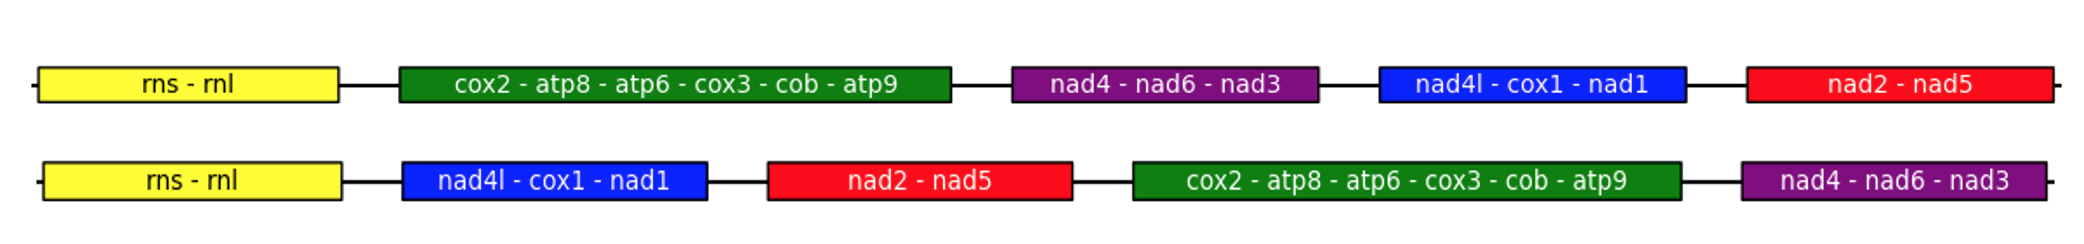
\includegraphics[width=1.0\textwidth]{Figures/figure 2.png}
    \caption{The two different configurations of gene orders seen in G3 and G4 sponges. In the 62 species studied, little variation was seen in this pattern until \emph{Niphates digitalis} and \emph{Niphates erecta}.}
\end{figure}

\begin{figure}[htp]
    \centering
    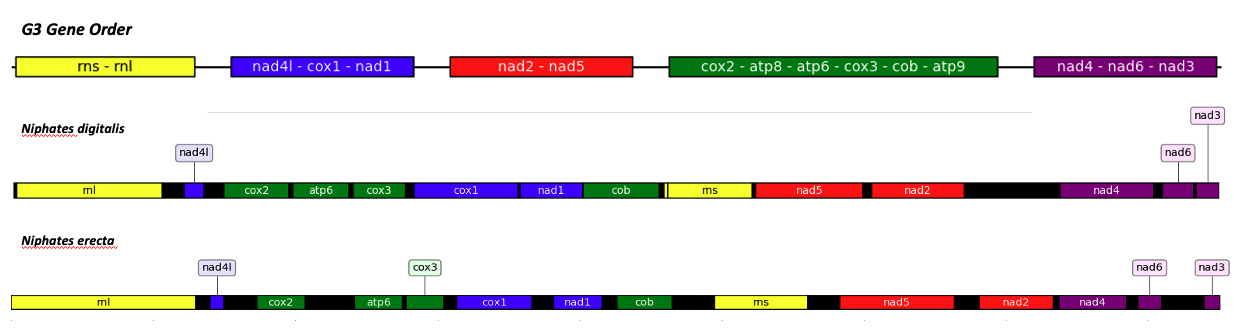
\includegraphics[width=1.0\textwidth]{Figures/figure 4.png}
    \caption{G3 gene order, color-coded, with the corresponding \emph{Niphates digitalis} and \emph{Niphates erecta} mt-genomes.}
\end{figure}

The five clusters alternate in pattern, with no cluster of NADH genes situated next to each other. As seen in Figure 2, G3 sponges show a pattern of the \emph{rnl} group, \emph{cox1} group, \emph{nad2} group, the \emph{cox2} group, and the \emph{nad4} group. Individual genes are typically separated by tRNA genes, but the identity of tRNA genes between genes is not consistent. When examining gene order, tRNA gene position was not considered.

The mitochondrial genomes for both \emph{Niphates} species do not match either pattern identified in G3 or G4, despite being most closely related to the G3 sponge \emph{Amphimedon queenslandica}. Multiple clusters have been rearranged, the \emph{Niphates} arrangements no longer bare any similarity to the gene orders seen in G3 and G4 sponges. To begin, \emph{rnl} and \emph {rns} are not found together, and instead are found with 8 and 6 genes on either side of them. The gene \emph{nad4l} has been separated from the \emph{cox1} group and is instead found by the \emph{cox2} group. The \emph{cox2} group appears to have been invaded by the \emph{cox1} group, as that group is now found in between \emph{cox3} and \emph{cob}. In addition, the \emph{nad2} group has been flipped, with \emph{nad5} appearing before \emph{nad2}. Finally, breaking the pattern of the NADH gene groups not appearing side-by-side, the \emph{nad4} group is found next to the flipped \emph{nad2} group. 

In terms of counted gene boundaries, \emph{Niphates digitalis} and \emph{Niphates erecta} have two less gene boundaries than expected for G3 sponges, which is a reflection of the two missing genes. G3 sponges are expected to have 16 different gene boundaries, while both \emph{Niphates} species have 14 gene boundaries. Of these 14 gene boundaries seen in \emph{Niphates}, 9 are not seen in the expected model for G3 sponges. However, one of these nine gene boundaries, \emph{cox2 - atp6}, is the direct result of the loss of \emph{atp8}, and not due to any proposed rearrangement. The other eight come be attributed to gene rearrangement.

\subsection{tRNA content and synthetases}
One of the novel traits seen in Clade B is a lack of mitochondrial tRNAs. The loss is seen in other sponges outside of Clade B, but Clade B represents an interesting example where some species have retained all of their mitochondrial tRNA genes while other species have lost many. On one end of the spectrum, \emph{Xestospongia muta} and \emph{Xestospongia testudinaria} have 26 mt-tRNA genes, including one gene that codes for an unknown tRNA, designated tRNA(X). They have lost no tRNA genes at all. On the other end of the spectrum lies the two \emph{Niphates} species; both mt-genomes have the same four mitochondrial tRNAs - Y, I, M, and W, and have lost all others. Between these are \emph{Amphimedon queenslandica} and \emph{Neopetrosia proxima}, each missing 7 and 4 tRNA genes respectively.

\subsection{Multiple insertions found in the \emph{N. erecta} mt-genome}

Until this point, the mt-genomes of \emph{Niphates digitalis} and \emph{Niphates erecta} have been shown to be near identical in terms of gene organization, genome content, nucleotide composition, and gene order. They are not without their differences, however. The primary difference between the two genomes lies in the novel insertions identified in the \emph{N. erecta} mt-genome. Eighty insertions have been identified in \emph{N. erecta} that are not seen in \emph{N. digitalis}, and range in size from a few base pairs to large sections up to 650 bps long. The majority of insertions fall into intergenic regions, and help account for the increase in total intergenic space seen in \emph{N. erecta}. However, there are also several insertions that fall into genes:\emph{cox2, atp6, nad1, nad5, rnl}, and \emph{rns}, of which \emph{cox2, atp6, nad1,} and \emph{nad5} are protein-coding.

As a few of these insertions fall into protein-coding genes, it was important to understand the impact, if any, these insertions have on down-stream products. The majority of insertions are in-frame, but two of these genes - \emph{atp6} and \emph{nad5} - have out-of-frame insertions. Although a \emph{Niphates erecta} proteome does not exist to determine if insertions are having effects on a protein level, the \emph{Niphates erecta} transcriptome provided an appropriate stand-in.

Multiple transcripts from the \emph{Niphates erecta} transcriptome were identified as containing the five protein-coding genes. Alignment of these transcripts with the mt-genome sequences shows that none of the transcripts have lost the insertions, and are therefore most likely present in the downstream protein.

\begin{center}
\begin{tabular}{ |c|c|c|c| } 
 \hline
 \textbf{Gene}& \textbf{Number of Inserts} & \textbf{In-Frame} & \textbf{Out-of-Frame}\\
 \hline
 \emph{cox2}  & 4  & 4 & 0 \\
\hline
\emph{atp6} & 5 & 4 & 1 \\
\hline
\emph{nad1} & 2 & 2 & 0 \\
\hline
\emph{nad2} & 1 & 1 & 0 \\
\hline
\emph{nad5} & 4 & 1 & 3 \\
\hline
\end{tabular}
\end{center}

Regardless of the impact these insertions and deletions have on proteins and downstream functions, they do account for the discrepancy in genomes size between species. The \emph{N. digitalis} and \emph{N. erecta} genomes are 25525 bps and 18285 bps, respectively. The majority of this length difference can be attributed to the increased number of intergenic regions and insertions seen in \emph{N. digitalis}. Intergenic regions account for 24.2\% of \emph{N. digitalis}'s genome, as opposed to 13.77\% in \emph{N. erecta}, and insertions in protein-coding areas account for an additional [INSERT PERCENTAGE HERE] of \emph{N. digitalis}'s mitochondrial genome.

\begin{figure}[htp]
    \centering
    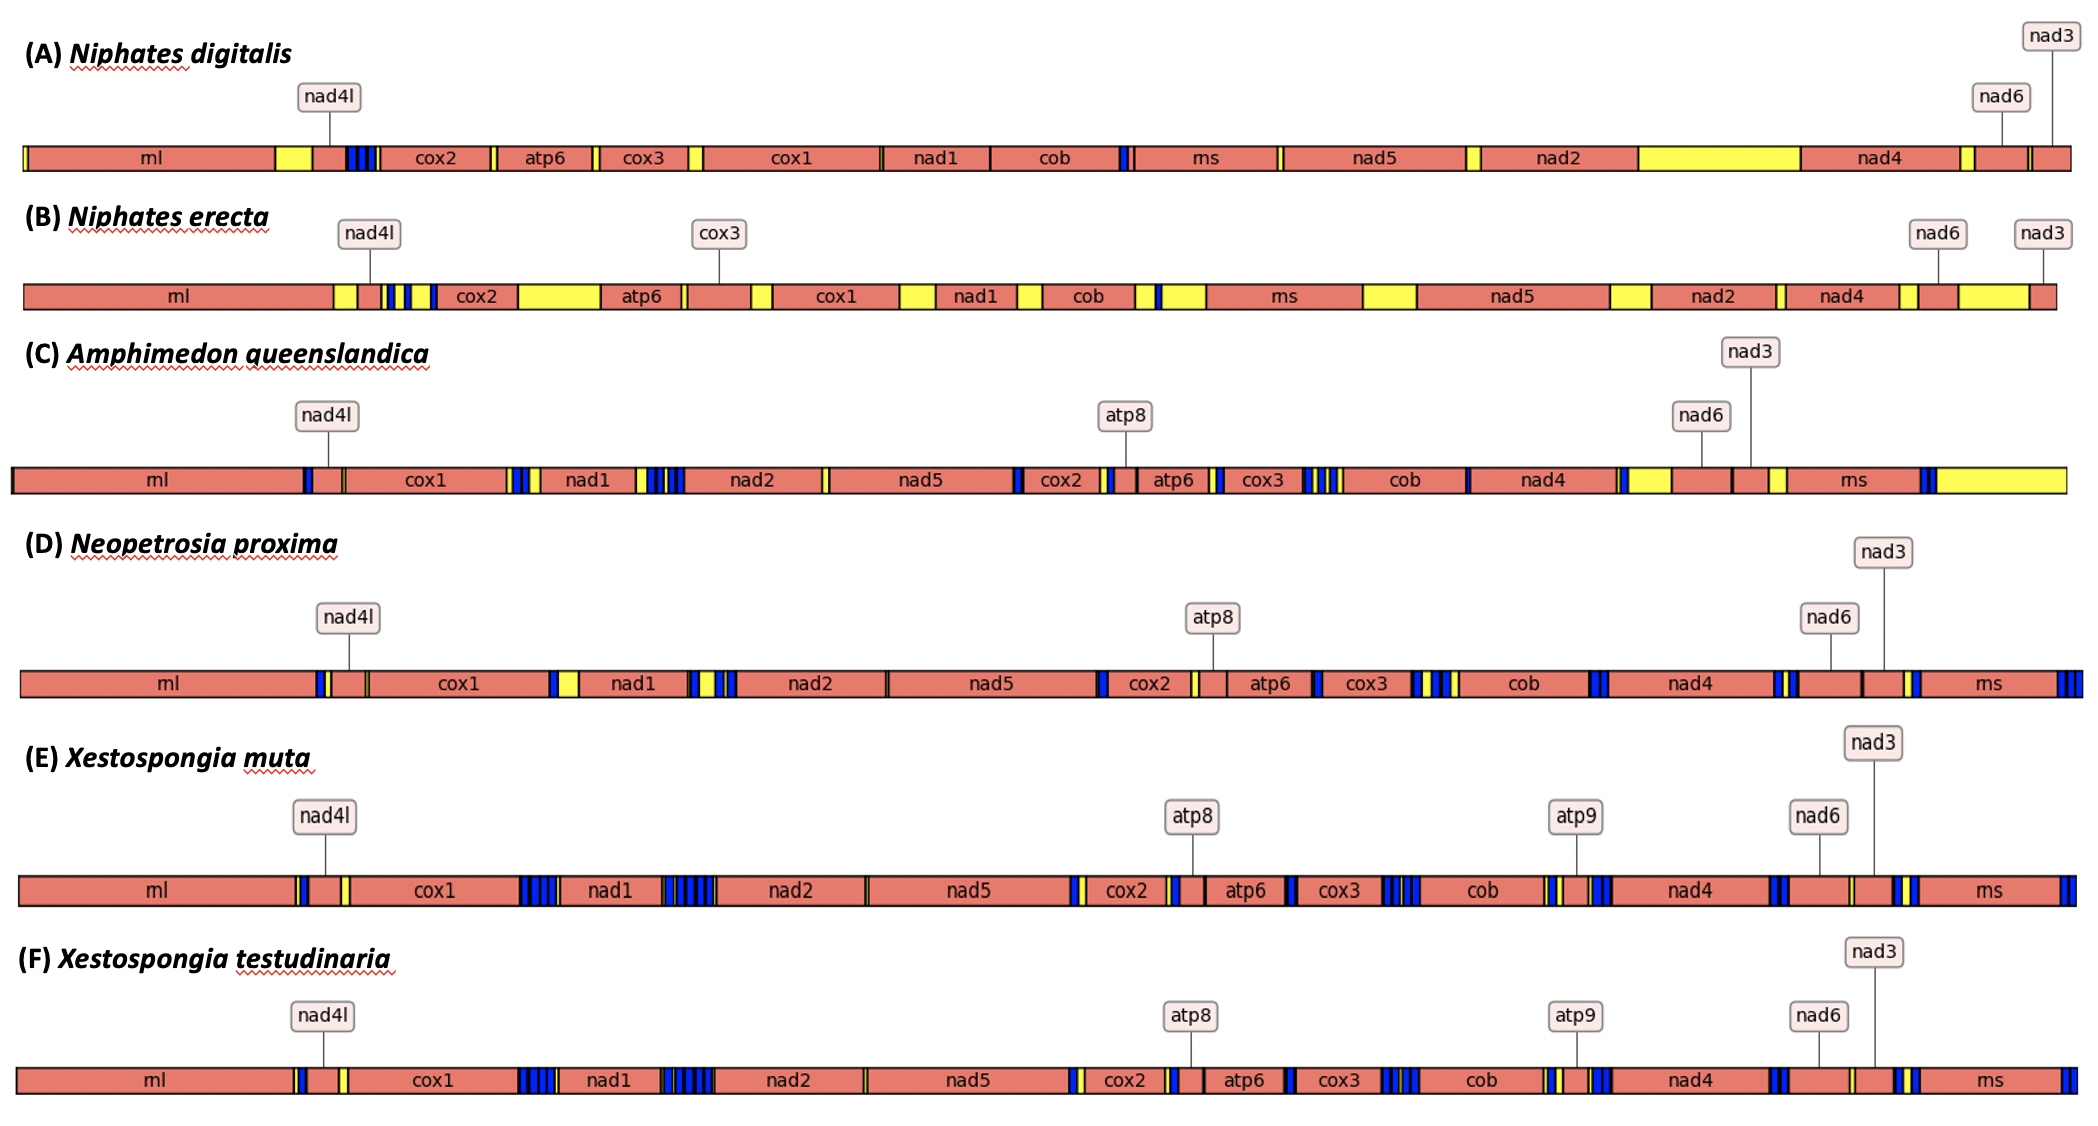
\includegraphics[width=1.0\textwidth]{Figures/figure 1.png}
    \caption{Red are coding genes, blue is tRNA genes, and yellow are intergenic regions. Purple bars above represent insertions in \emph{Niphates erecta} versus \emph{Niphates digitais}, while the green bars represent stem-loop elements.}
\end{figure}

\subsection{Inverted Repeats}

Further analysis of \emph{N. digitalis}'s insertions and intergenic regions found that many contain inverted repeat sequences. The locations of these can be seen in Figure Y. Inverted repeats have previously been identified in other sponge species, and their function is unknown. These inverted repeats were isolated from the genome, and like the insertions, analyzed with NCBI BLAST. They returned no close sequence relations under any parameters. Alignments of the \emph{Niphates} inverted repeats showed that majority of repeats have the same general sequence, see Figure 6, and when folded form hairpin-like structures.

The inverted repeats fall into four different motifs, the structures of which can be seen in Figure 6. The majority of inverted repeats contain motif 1. Motif 1 contains a highly conserved 11-nucleotide stem with a 4 nucleotide loop. Before and after the stem-loop is not conserved. Motif 2 shows a similar pattern, though it is less common. It contains a well-conserved 12 nucleotide stem with a 3 nucleotide loop at the top. In addition, bases before the stem-loop are typically conserved. Motif 3 is another large, well conserved stem-loop, with a 13 base stem and a six nucleotide loop. As with the others, the regions on either side of the stem are not conserved. Motif 4 is much smaller, with a 5 nucleotide stem and a 6 nucleotide loop. 

Many of the inverted repeats appear and stem-loop elements appear in a large sections together, results in dense regions of stem-loop elements. The function of these stem-loop elements is unknown. In addition, the same motifs appear at different points across the genome, and do not group together in particular locations.

Analysis of the other mt-genomes in Clade B reveal no other stem-loops or inverted repeats, making these traits unique to \emph{Niphates erecta}.

\begin{figure}[htp]
    \centering
    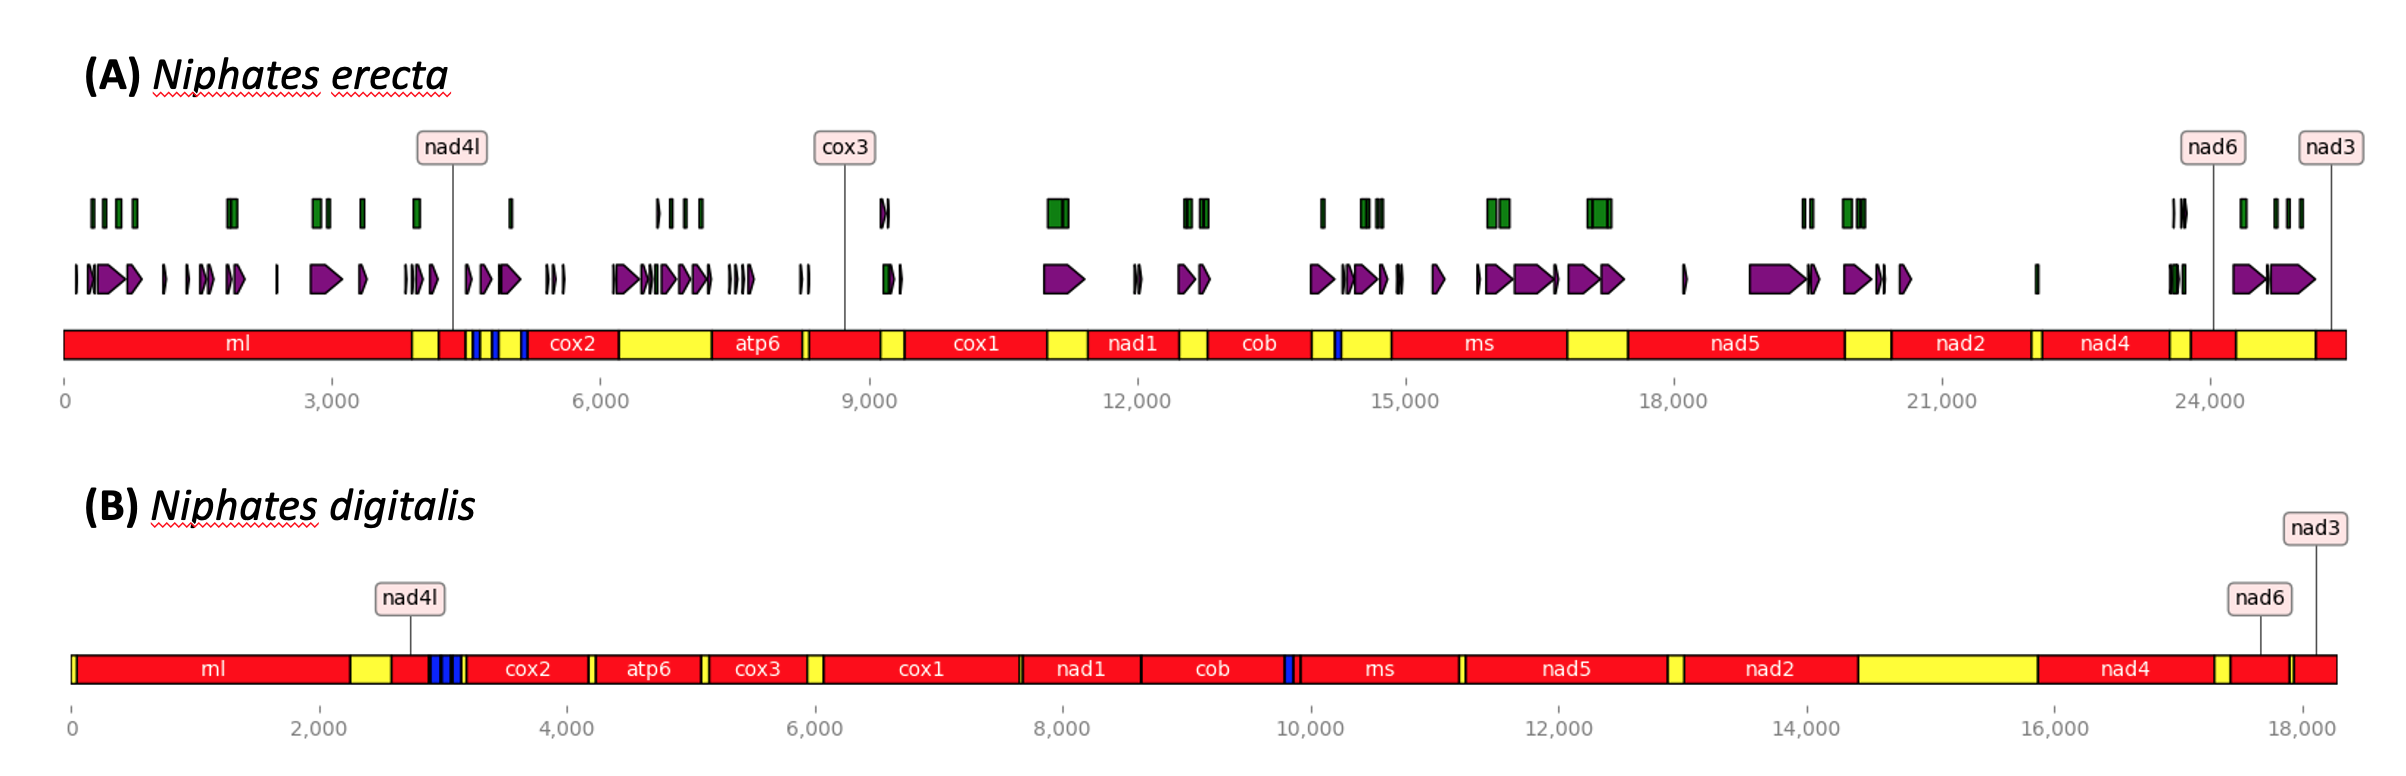
\includegraphics[width=1.0\textwidth]{Figures/figure 5.png}
    \caption{Red are coding genes, blue is tRNA genes, and yellow are intergenic regions. Purple bars above represent insertions in \emph{Niphates erecta} versus \emph{Niphates digitais}, while the green bars represent stem-loop elements.}
\end{figure}

\end{document}